\documentclass{article}
\usepackage{graphicx} % Required for inserting images
\title{Rapport MIN SET COVER \emph{online}}
\author{Georg Dorndorf, Louis Milhaud \& Niranjan Nair}
\date{February 2024}

\begin{document}

\maketitle

\section{Problem}
\textbf{Input:}
\begin{itemize}
    \item a set universe $U = \{0, 1, ..., n-1\}$
    \item a collection $S$ of $m$ subsets $S_i$ of $U$ such that $\bigcup\limits_{i = 0}^m S_i = U$
    \item a sequence $\sigma$ of size $k$ of elements of $U^* \subseteq U$
\end{itemize}
\textbf{Objective:}\\
Find a collection $S' \subseteq S$ such that $\sigma$ is covered at all time and $|S'|$ is minimum.

\section{Algorithms}
$\forall\ 0 \leq i \leq k$ let $C_i \subseteq S$ be the collection of sets containing $\sigma_i$.\\
\subsection{Full random algorithm}
\textbf{Description:}\\
$\forall\ 0 \leq i \leq k$:\\
If $\sigma_i$ is already covered, we go to the next element in the sequence.\\
Else we randomly select a set in $C_i$.

\subsection{Biggest cover algorithm}
\textbf{Description:}
$\forall\ 0 \leq i \leq k$:\\
If $\sigma_i$ is already covered, we go to the next element in the sequence.\\
Else we select $S_\diamond\in C_i$ such that $S_\diamond$ contains the most uncovered elements:
$$|S_\diamond| = \max_{0\leq j\leq m}\{|S_j| - |S_j\cap S'|\}$$ with $S'$ the current cover.\\

We also wrote the \emph{smallest cover algorithm} just for comparison reasons, it's a dual to this algorithm.\\

The two algorithms we saw have the same worst-case complexity, both of them can have: $|S'| = |U^*|$.
The following input is a valid example:
\begin{itemize}
    \item[-] $|U| = 7$
    \item[-] $S = \{\{0, 3, 4, 5, 6\}, \{0, 1, 3, 4\}, \{0, 1, 2\}\}$
    \item[-] $\sigma = [0, 1, 2]$
\end{itemize}
Both of them can have $S$ as an answer.
\subsection{Log algorithm}
\textbf{Description:}

\section{Competitivity}
\hspace*{-2in}
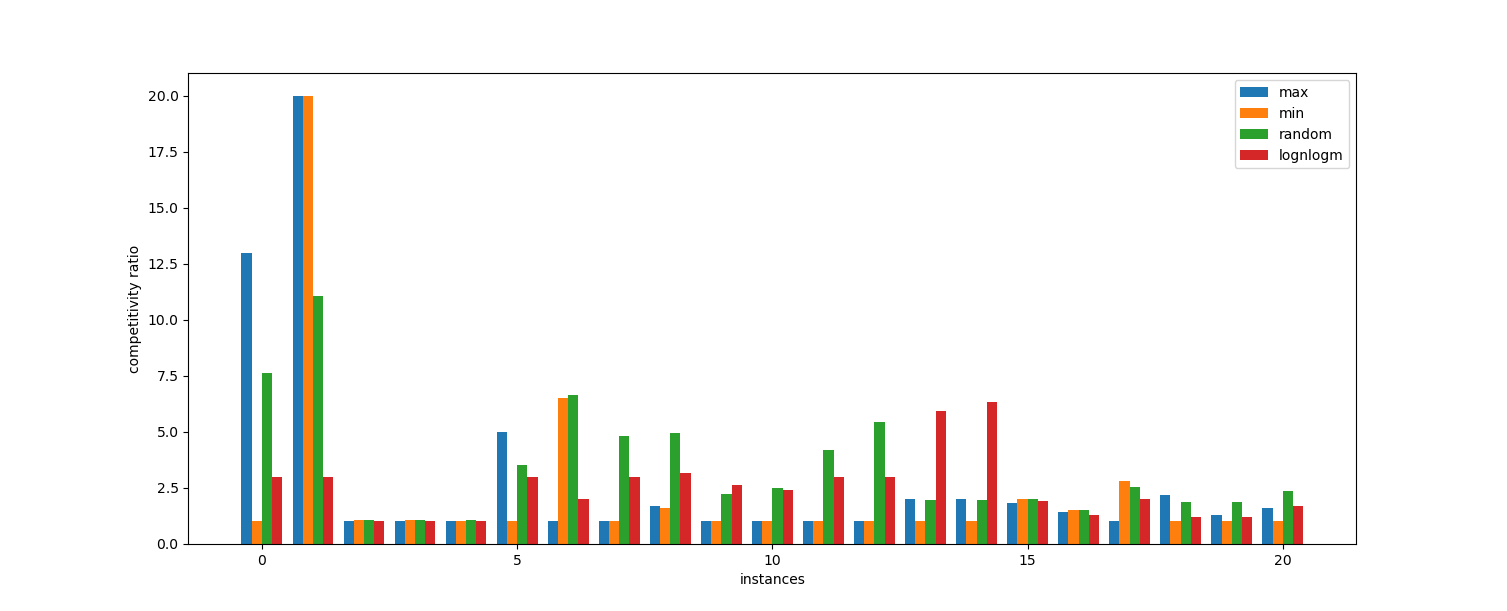
\includegraphics[scale=0.6]{competitivity ratio.png}

We observe that the best algorithm it's often the \emph{lognlogm} algorithm, which could be expected since it has very good theoretical results. Nonetheless, this wasn't clear in a previous plot where only the cost was displayed: for small instances like we have the cost of complex algorithms that are good in theory can be very high. We also observe that some instances are more difficult than others, causing huge competitive ratios (20 !) for the \emph{min} and \emph{max} algorithm. Because of that, the \emph{full random} algorithm shows some resiliency and may appear as a good naive approximation. Finally, we're very surprised that the \emph{min} algorithm shows better results than \emph{max} algorithm, showing that the instances are very specific.
% TODO: 95% interval for the best + observations
\end{document}
